\section{Motivation}
\myblockquote{
A display connected to a digital computer gives us a chance to gain familiarity with concepts not realizable in the physical world. It is a looking glass into a mathematical wonderland. (Ivan Sutherland, 1965)
}{\cite{sutherland1965ultimate}}

\begin{figure}[h!]
\centering
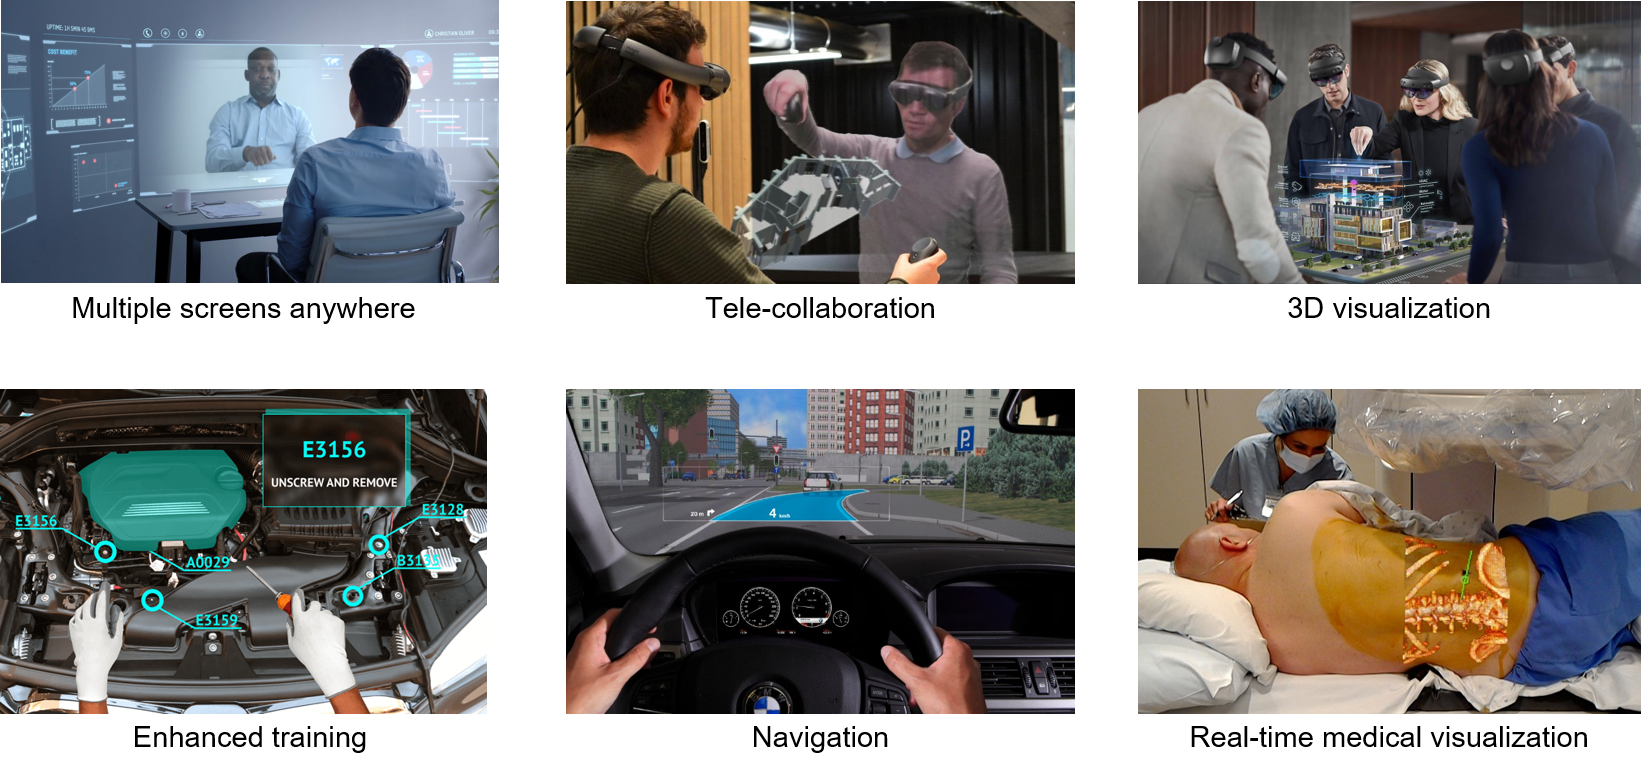
\includegraphics[width=\columnwidth]{images/other/motivation}
\caption[Motivation for Augmented Reality]{Augmented Reality provides new and better methods to communicate and visualize. 
Figure shows some envisioned applications. Image credits are given below:\\
\footnotesize
\emph{(top,left):} \href{https://www.pinterest.com/pin/353462270745212902/}{https://www.pinterest.com/pin/353462270745212902/}\\
\emph{(top,middle):} \href{https://www.mimesysvr.com/}{https://www.mimesysvr.com/}\\
\emph{(top,right):} \href{https://medium.com/cgi-norway/augmented-reality-in-business-and-future-for-consumers-d4b8fcdee4a6}{https://medium.com/cgi-norway/augmented-reality-in-business-and-future-for-consumers-d4b8fcdee4a6}\\
\emph{(bottom,left):} \href{https://www.growthbusiness.co.uk/uk-based-ar-firm-makes-largest-ar-fundraise-of-the-year-2555730/}{https://www.growthbusiness.co.uk/uk-based-ar-firm-makes-largest-ar-fundraise-of-the-year-2555730/}\\
\emph{(bottom,middle):} \href{https://www.driversalert.com/augmented-reality-heads-up-display-distracted-driving/}{https://www.driversalert.com/augmented-reality-heads-up-display-distracted-driving/}\\
\emph{(bottom,right):} \href{https://hololens.reality.news/news/hololens-assists-live-surgery-0178887/}{https://hololens.reality.news/news/hololens-assists-live-surgery-0178887/}\\
%\footnote{URL: \href{https://www.forbes.com/sites/charliefink/2019/12/10/magic-leap-drops-news-bombs-about-enterprise-updates-and-magic-leap-2/\#613142941263}{https://www.forbes.com/sites/charliefink/2019/12/10/magic-leap-drops-news-bombs-about-enterprise-updates-and-magic-leap-2/\#613142941263}} 
%\footnote{URL: \href{https://medium.com/cgi-norway/augmented-reality-in-business-and-future-for-consumers-d4b8fcdee4a6}{https://medium.com/cgi-norway/augmented-reality-in-business-and-future-for-consumers-d4b8fcdee4a6}}
%\footnote{URL: \href{https://www.growthbusiness.co.uk/uk-based-ar-firm-makes-largest-ar-fundraise-of-the-year-2555730/}{https://www.growthbusiness.co.uk/uk-based-ar-firm-makes-largest-ar-fundraise-of-the-year-2555730/}}
%\footnote{URL: \href{https://www.driversalert.com/augmented-reality-heads-up-display-distracted-driving/}{https://www.driversalert.com/augmented-reality-heads-up-display-distracted-driving/}}
%\footnote{URL: \href{https://hololens.reality.news/news/hololens-assists-live-surgery-0178887/}{https://hololens.reality.news/news/hololens-assists-live-surgery-0178887/}}
}
\label{fig:motivation}
\end{figure}



The goal of Augmented Reality is to seamlessly integrate the real world and the digital world.
Although Augmented Reality hopes to address the combination of real and digital worlds for all our sense-modalities, i.e., sight, smell, touch, and hearing, in this dissertation, we shall only consider Augmented Reality for sight. 
There has been significant progress over the decades to create synthetic photorealistic imagery for movies, games, etc. 
But until recently, the most common way to interact with digital worlds was through 2D displays such as televisions, computer monitors, or mobile phones and tablets. 
These displays are 2D displays and subtend a narrow field-of-view. 
Since we live in a 3D world and our eyes see a wide field-of-view image, today’s displays severely limits our communication, visualization, and interaction with the digital world. 
Providing a seamless, perceptually realistic experience requires more than just rendering photorealistic imagery. 
It requires display that can present wide field-of-view high-quality imagery, and in particular, it requires that these displays support all depth cues of the human visual system (Palmer, 1999; Howard and Rogers, 2002) accurately. 
Display technologies that enable a seamless combination of the real and digital worlds could revolutionize the way we communicate, visualize and interact with digital information.
Fig. \todo{rename} shows some compelling envisioned applications for future Augmented Reality systems.

\paragraph{Multiple screens anywhere:} an AR system can not only fully replace our current 2D displays (televisions and computer monitors), but can place virtual versions of our 2D displays any location around us. 
The future workspace would be more customizable and productive than ever before.
\paragraph{Tele-collaboration:} an AR system with AR displays and 3D reconstruction system can enable an advanced version of today’s video teleconferencing. 
In the envisioned system, the remote AR system would capture the remote person’s geometry and colors and transmit it to the local AR system which would render the remote person such that they appear to be in the local physical space. 
\paragraph{3D visualization:} future AR system would enable us to visualize 3D structures and volumetric effects (fog, fluid simulations, etc.) in very informative ways. 
Sometimes, future AR systems may even be better than recreating such 3D structures in the real-world because in a digital system, we could have the option to visualize not just the structure as a whole, but informative versions of the structure, e.g., cross-sectional view, part-wise view, etc. 
\paragraph{Enhanced training:} it has already been demonstrated that spatially registered training programs and manuals improve learning rate[To do: needs citation]. 
\paragraph{Navigation:} Similar to the point above, navigation is another example of contextual information that can be presented better with an AR display because it is spatially registered to where the user is already looking.
\paragraph{Real-time medical visualization:} one of the most important applications for future AR is probably in medical sciences, e.g., spatially registering visualization of the internal organs of the current patient underoing a surgery.

\section{Scope of this dissertation}
\begin{figure}[h!]
\centering
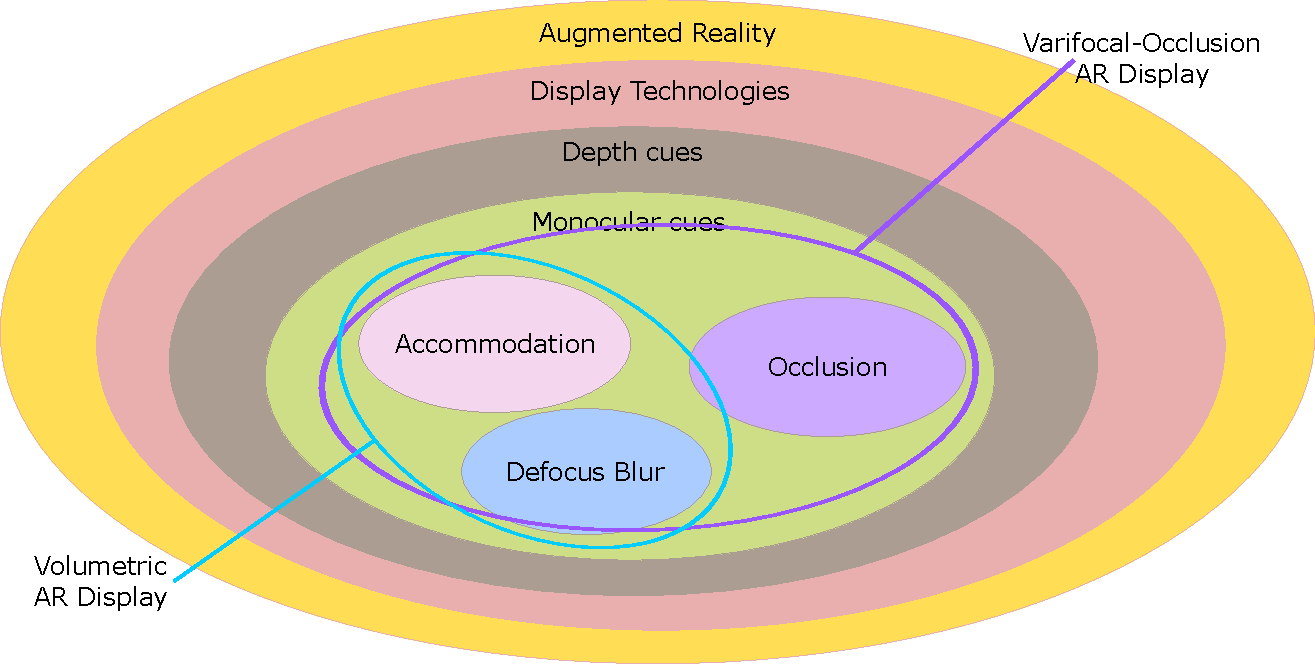
\includegraphics[width=\columnwidth]{images/other/scope}
\caption[Scope of this dissertation]{Figure shows the scope of this dissertation.}
\label{fig:scope}
\end{figure}


Fig. \todo{rename} depicts the scope of this dissertation. 
There are many enabling technologies and active research areas for Augmented Reality e.g., display technologies, 3D reconstruction, tracking, virtual assistants, redirected walking, etc. 
This dissertation focusses on display technologies. 
Even for just the topic of display technologies, there are a number of disserata outlined in Sec. \todo{rename}. 
This dissertation considers only three specific monocular depth cues, namely: occlusion, accommodaiton and defocus-blur. 
These depth-cues are explained and dicussed in-detail in Sec. \todo{rename}, but briefly, these three depth cues are important monocular depth cues whose absense in AR displays has demonstrated reduced task performance \todo{needs citation} and increased discomfort \todo{needs citations}. 
For these depth cues, this dissertation develops two display technologies that improve the presentation of these depth cues over a large depth-range.


\section{Thesis Statement}
The use of computational displays, where the optics, electronics, and algorithms are co-designed, will improve accommodation, defocus-blur, and occlusion in AR displays.

\section{Contributions of this dissertation}
For accommodation and retinal-blur, this dissertation’s contributions are: 
(1) A volumetric NED exhibiting 280 perceptually simultaneous binary depth planes, each an arbitrary RGB color, situated between 15 cm (6.7 diopters) and 400 cm (0.25 diopters) from the viewer. 
(2) A rendering pipeline that decomposes a 3-D scene into the set of single-color binary depth planes, such that 24 bpp color voxels are displayed at 280 unique depth positions. 
(3) A yet-to-be-developed color-adaptive decomposition algorithm for the NED which also demonstrates intra-pupillary occlusions. 

For depth-dependent occlusion, accommodaiton, and retinal blur, this dissertation’s contributions are: 
(1) Varifocal occlusion as an AR display capability that adaptively changes the focal distance of an occlusion mask to enable depth-dependent hard-edge occlusion. 
(2) Complementary approaches of optimization and closed-form solutions for arriving at an optical design that enables a focus-tunable optical system to achieve varifocal occlusion in a perceptually realistic manner without optically distorting the observed scene. 
(3) A monocular varifocal occlusion-capable AR display prototype that demonstrates depth-dependent occlusion over a large depth range (30 cm to 300 cm). 

The broad contributions of this dissertation are new optical designs, new real-time rendering algorithms, and prototype displays that demonstrate monocular depth-cues such as accommodation, defocus-blur, and hard-edge occlusion over a large depth-range. 